\documentclass[12pt,]{article}
\usepackage[utf8]{inputenc}
\usepackage[T1]{fontenc}
\usepackage{mathptmx}
\usepackage{geometry}
\usepackage{mathtools}
\usepackage[english]{babel}
\usepackage{graphicx}
\usepackage{subcaption}
\usepackage{stackengine}
\usepackage[os=win]{menukeys}
\usepackage{hyperref}
\usepackage{minted}
\usepackage{xcolor}
\usepackage{tikz}
\usepackage[yyyymmdd,hhmmss]{datetime}
\usepackage{etoolbox}
\usepackage[inline]{enumitem}
\usepackage{pdfpages}

\newcommand{\WindowsLogo}{\raisebox{-0.1em}{
\includegraphics[height=0.8em]{images/logo/Windows_3_logo_simplified}}}
%\newcommand{\PowerLogo}{\raisebox{-0.1em}{\includegraphics[height=0.8em]{images/logo/power}}}
\newcommand{\WinKey}{\keys{\WindowsLogo}}
\newcommand{\PowerKey}{\keys{\PowerLogo}}

\patchcmd{\thebibliography}{\section*{\refname}}{}{}{}

\newcommand{\ShowOsVersion}{
	\immediate\write18{\unexpanded{foo=`uname -sro` && echo "${foo}" > tmp.tex}}
	\input{tmp}\immediate\write18{rm tmp.tex}
}

\newcommand{\ShowTexVersion}{
	\immediate\write18{\unexpanded{foo=`pdflatex -version | head -n1 | cut -d' ' -f1,2` && echo "${foo}" > tmp.tex}}
	\input{tmp}\immediate\write18{rm tmp.tex}
}

\addto\captionsenglish{\renewcommand{\contentsname}{Daftar Isi}}
\addto\captionsenglish{\renewcommand{\figurename}{Gambar}}

\hypersetup{
	colorlinks=true, %set true if you want colored links
	linktoc=all,     %set to all if you want both sections and subsections linked
	linkcolor=blue,  %choose some color if you want links to stand out
	urlcolor=blue,   %url color
}

\geometry{
	a4paper,
	left=10mm,
	right=10mm,
	top=10mm,
	bottom=15mm,
}

\title{\LARGE \bf
	Laporan Pengujian Unit Speech/Whisper Tester\\
}

\author{Achmadi ST MT}

\date{}

\hypersetup{citecolor=black}

\definecolor{LightGray}{gray}{0.95}

%\pagecolor[rgb]{0.1,0.1,0.1}
%\color[rgb]{1,1,1}

\begin{document}
	\thispagestyle{empty}
	
	\begin{titlepage}
		\centering
		\vfill
		\vfill
		\maketitle
		\vfill
		
\includegraphics[width=200pt]{images/logo/logoviblab}
		\vfill
		\vfill
		Update: {\today} \currenttime \\
	\end{titlepage}
	
	%%%%%%%%%%%%%%%%%%%%%%%%%%%%%%%%%%%%%%%%%%%%%%%%%%%%%%%%%%%%%%%%%
	
	\newpage
	\tableofcontents
	
	%%%%%%%%%%%%%%%%%%%%%%%%%%%%%%%%%%%%%%%%%%%%%%%%%%%%%%%%%%%%%%%%%
	
	\newpage
	\section{Pendahuluan}
	
	\subsection{Tujuan}
	
	Tujuan kegiatan pengukuran ini meliputi:
	\begin{itemize}
		\item Mengetahui nilai dB SPL untuk Elitech Speech Test menggunakan Headphone
		\item Mengetahui nilai dB SPL untuk Elitech Wishper Test menggunakan Headphone
		\item Mengetahui nilai dB SPL untuk Elitech Speech Test menggunakan Speaker
		\item Mengetahui nilai dB SPL untuk Elitech Wishper Test menggunakan Speaker
	\end{itemize}
	
	\subsection{Waktu dan Tempat}
	
	Seluruh kegiatan dilakukan di Ruang Semi-Unechoic Laboratorium Vibrasi dan Akustik
	Departemen Teknik Fisika Institut Teknologi Sepuluh Nopember Surabaya.
	
	%%%%%%%%%%%%%%%%%%%%%%%%%%%%%%%%%%%%%%%%%%%%%%%%%%%%%%%%%%%%%%%%%
	
	\newpage
	\section{Persiapan}
	
	Kegiatan persiapan disini meliputi:
	\begin{itemize}
		\item Modifikasi file Audio.
		\item Kalibrasi instrumen ukur.
		\item Pengukuran audio latar ruangan.
	\end{itemize}

	Instrumen yang digunakan meliputi:
	\begin{itemize}
		\item miniDSP EARS, berupa replika telinga karet dengan mikrofon, box DSP, dan antarmuka USB.
		Website produk:\\
		\url{https://www.minidsp.com/products/acoustic-measurement/ears-headphone-jig}
		
		\begin{figure}[!ht]
			\centering
			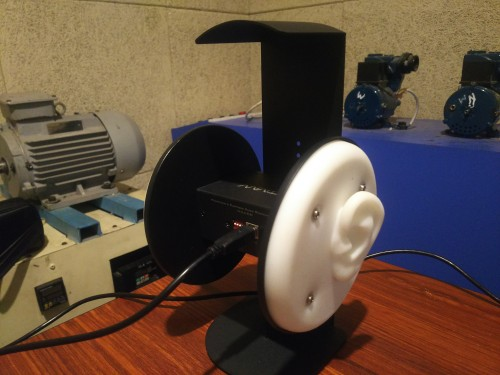
\includegraphics[width=200pt]{images/ears}
			\caption{miniDSP EARS}
		\end{figure}
	
		Untuk selanjutnya, paket intrumen ini disebut EARS saja.
		
		\item Focusrite dan Microphone (menyusul)
		
		Untuk selanjutnya paket instrumen ini disebut Mic saja
		
		\item Pistonphone Calibrator IEC942 dengan frekuensi 1000Hz dan loudness 114dB SPL sebagai acuan kalibrasi.
		\begin{figure}[!ht]
			\centering
			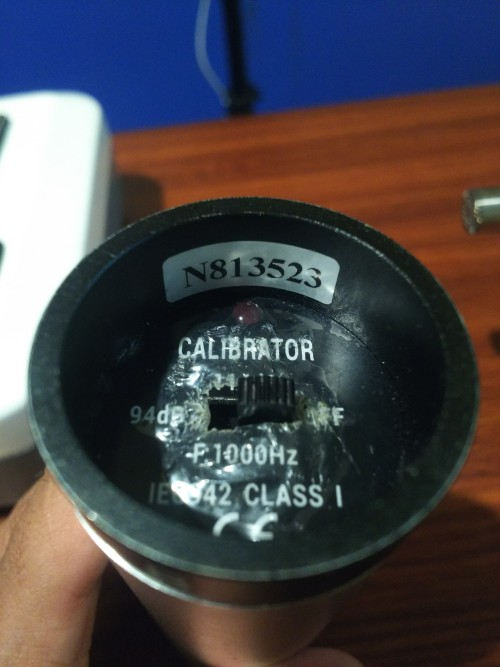
\includegraphics[width=150pt]{images/calibrator}
			\caption{Calibrator}
		\end{figure}
	
		\item SLM Onnosokki sebagai pembanding dalam pengukuran latar.
		SLM telah terkalibrasi dan telah dicek dengan kalibrator.
		Untuk selanjutnya paket instrumen ini disebut SLM saja.
		
		\newpage
		\begin{figure}[!ht]
			\centering
			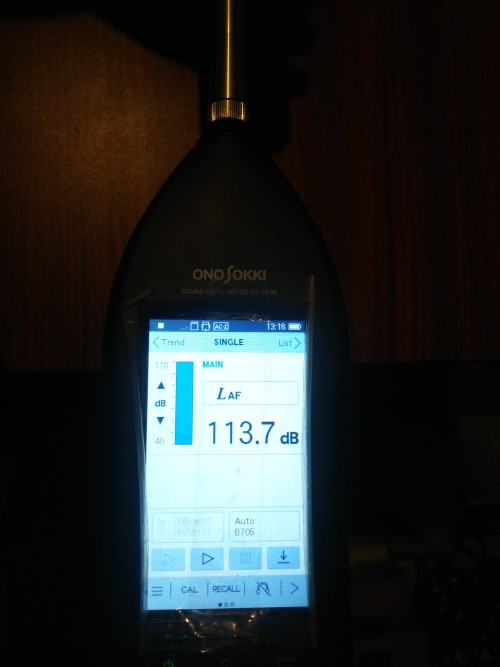
\includegraphics[width=150pt]{images/slm_calib}
			\caption{SLM Onnosokki}
		\end{figure}
		
	\end{itemize} 

	\subsection{File Audio}
	
	Dalam SDCard yang terinstal di unit prototype, tersedia 20 file audio MP3 dengan pembagian:
	\begin{itemize}
		\item File nomor 01 hingga 10 untuk Speech Test.
		\item File nomor 11 hingga 20 untuk Wishper Test.
	\end{itemize}

	Dipilih file 01 dan 11.
	Kemudian kedua file tersebut dibuang \textit{silence} di antara 5 kata pertama.
	Selanjutnya sisa \textit{track} dibuang.
	Tujuannya adalah untuk bisa diputar \textit{looping} dengan meminimumkan \textit{silence}.
	
	\begin{figure}[!ht]
		\centering
		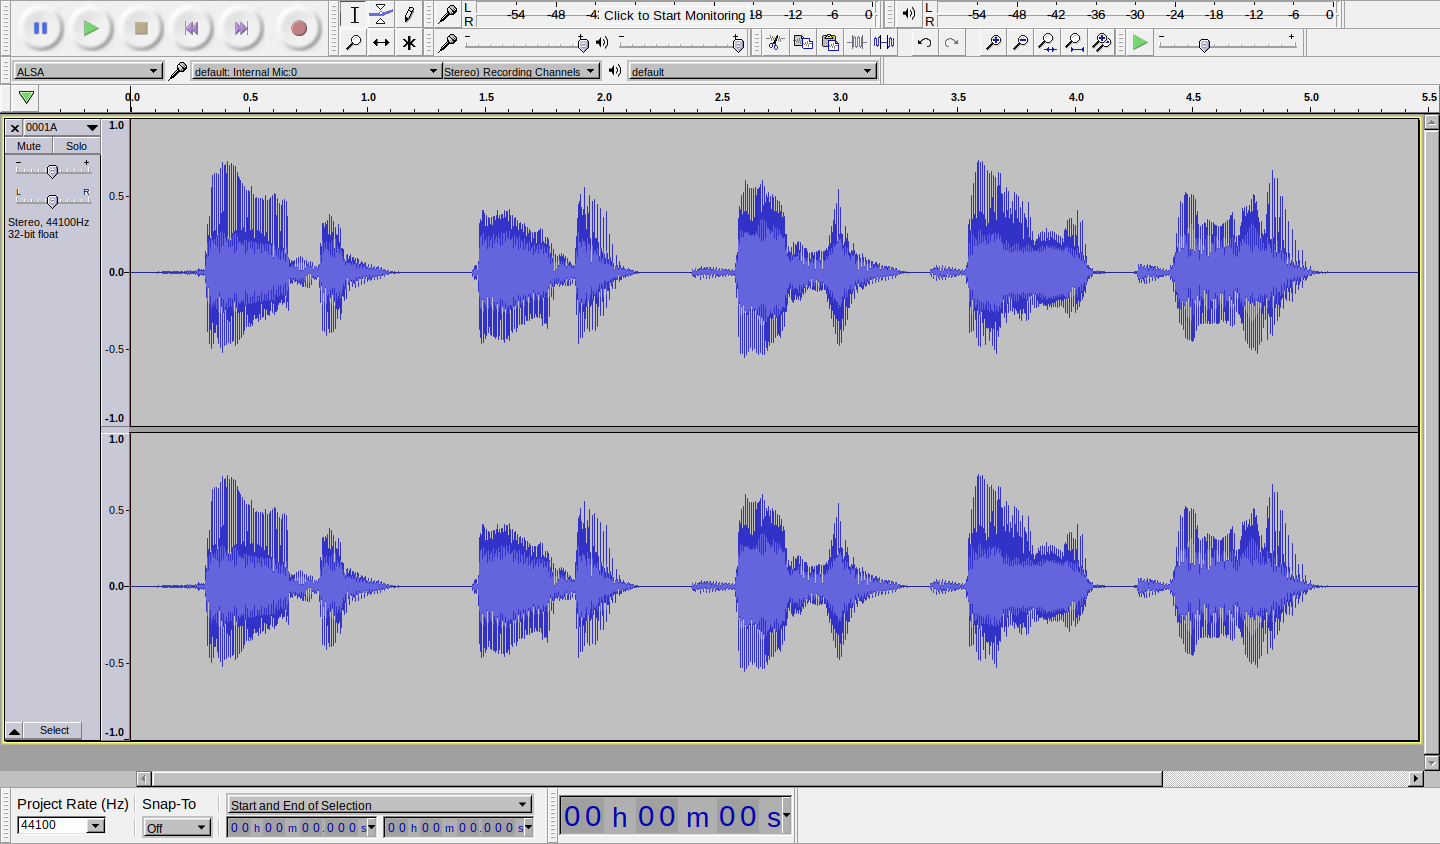
\includegraphics[width=250pt]{images/elitech_testAudioSpeech}
		\caption{Track Audio untuk Speech}
	\end{figure}

	\begin{figure}[!ht]
		\centering
		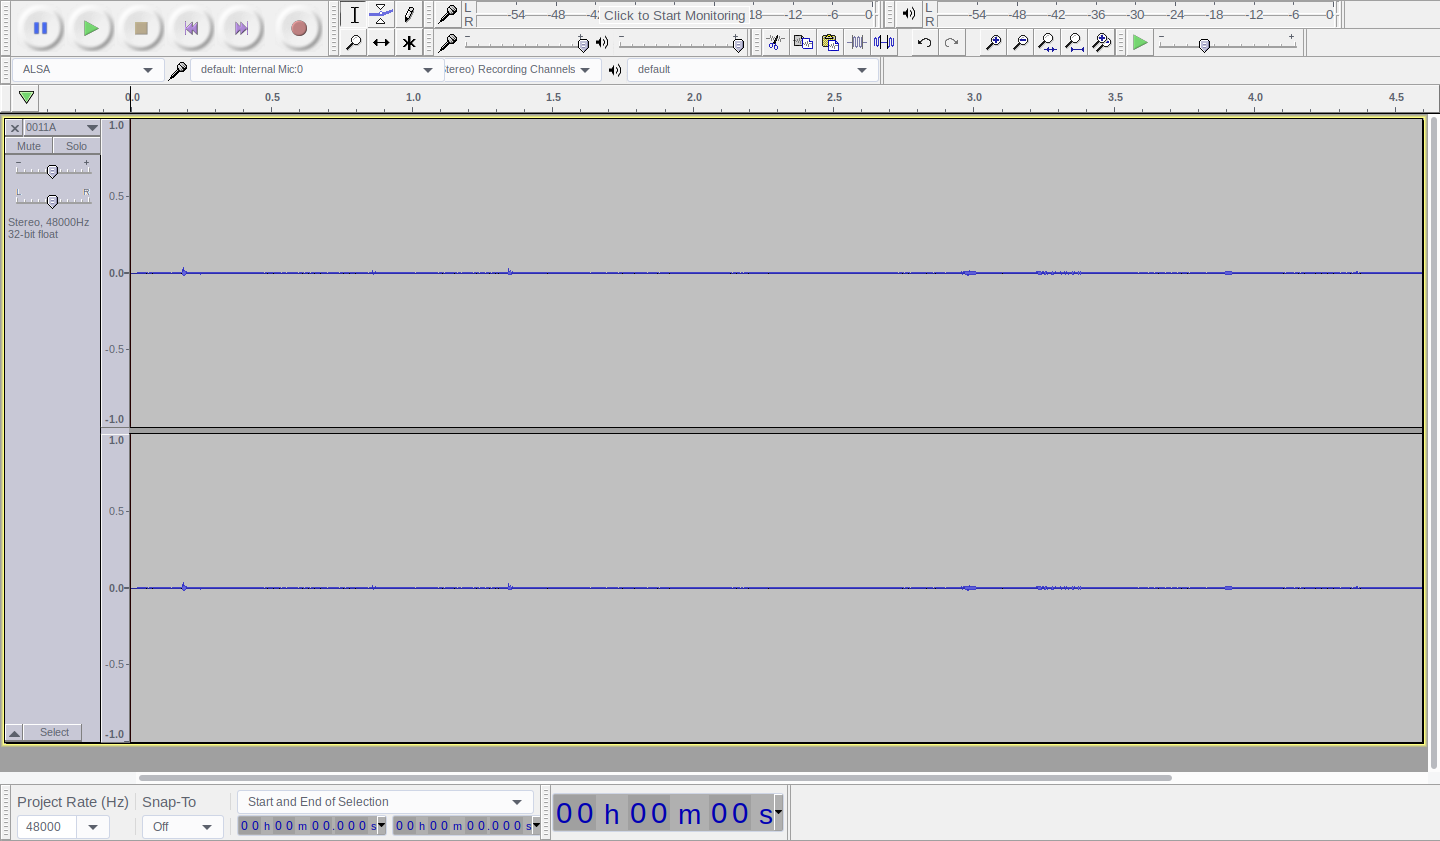
\includegraphics[width=250pt]{images/elitech_testAudioWhisperOri}
		\caption{Track Audio untuk Whisper}
	\end{figure}
	
	\newpage
	Perlu diketahui bahwa Audio Whisper memiliki level bit sangat rendah mendekati silence.
	
	\begin{figure}[!ht]
		\centering
		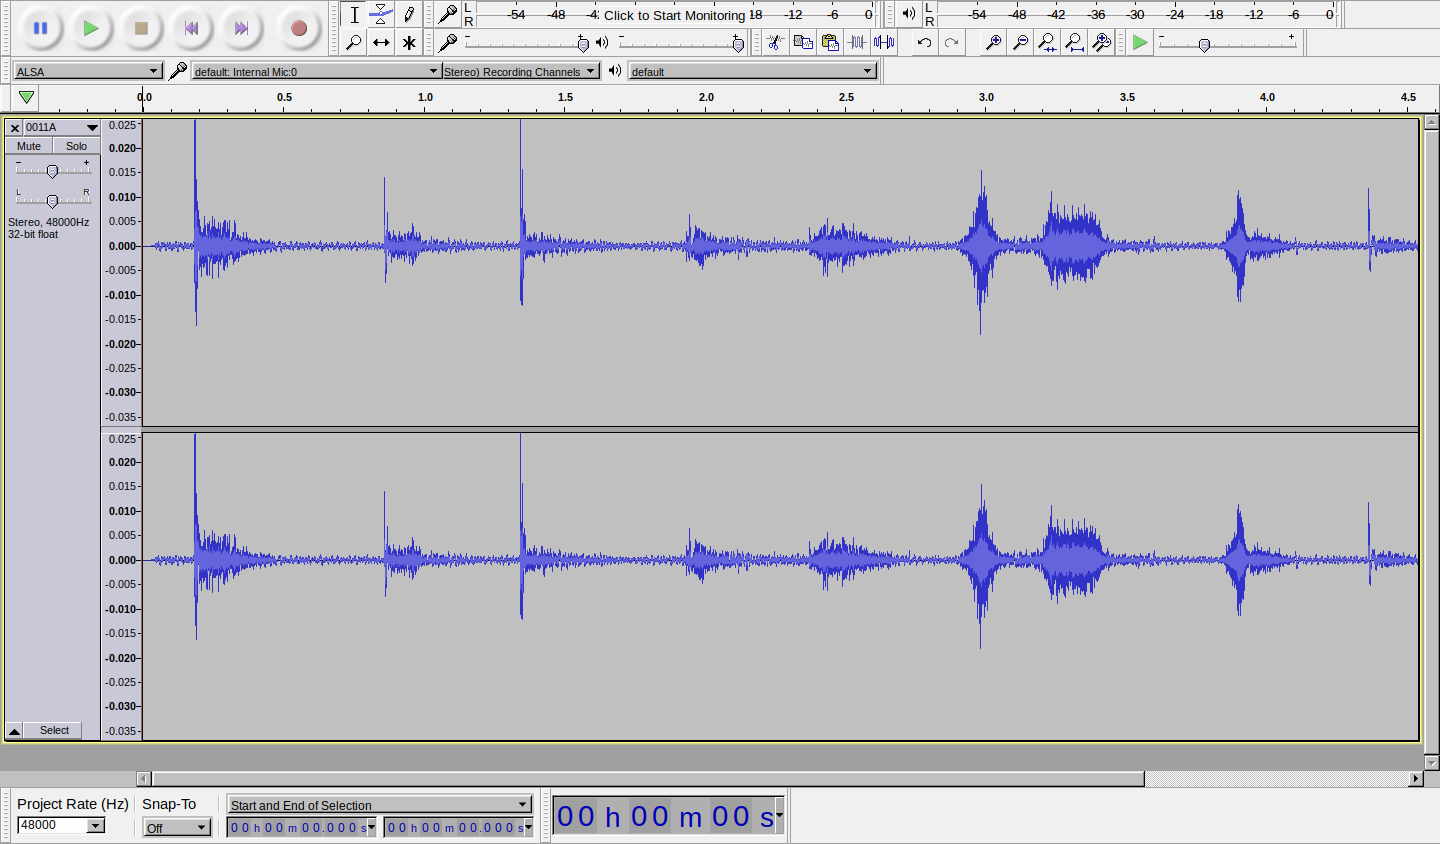
\includegraphics[width=250pt]{images/elitech_testAudioWhisper}
		\caption{Track Audio untuk Whisper (Zoomed)}
	\end{figure}

	Kemudian melihat analisa frekuensi:
	
	\begin{figure}[!ht]
		\centering
		\begin{subfigure}[b]{0.3\textwidth}
			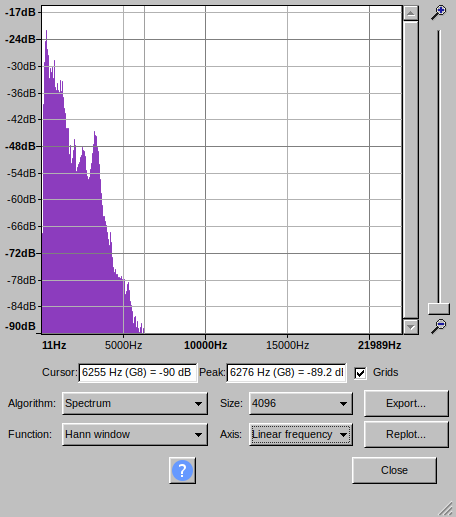
\includegraphics[width=\textwidth]{images/elitech_testAudioSpeechFreq}
			\caption{Speech}
		\end{subfigure}
		\begin{subfigure}[b]{0.3\textwidth}
			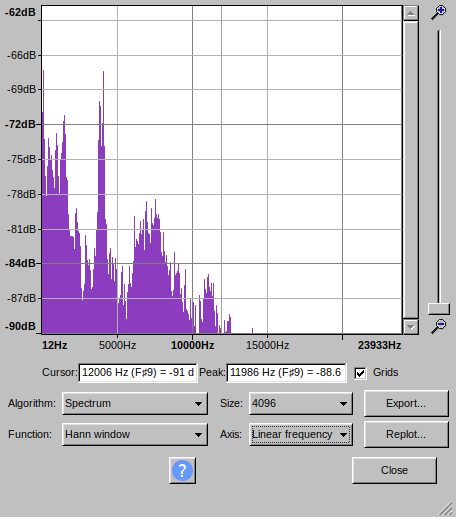
\includegraphics[width=\textwidth]{images/elitech_testAudioWhisperFreq}
			\caption{Whisper}
		\end{subfigure}
		\caption{Analisa Frekuensi}
	\end{figure}

	Disini diambil rentang \textit{upper-frequency} adalah 12500 Hz,
	sedangkan untuk frekuensi rendah diambil semua namun dengan pembobotan \textbf{A-Weighting}
	untuk mengurangi derau yang umumnya berada di frekuensi rendah.
	
	\subsection{Kalibrasi}
	
	Proses kalibrasi dilakukan untuk dua paket intrumen, yaitu EARS dan Mic.
	
	\subsubsection{EARS}
	
	Langkah kalibrasi EARS meliputi:
	\begin{enumerate}
		\item Lepas semua telinga karet sehingga internal microphone bisa ter-\textit{expose}
		\item Pastikan semua switch diatur untuk gain 0dB.
		\item Sambungkan USB ke laptop.
		\begin{enumerate}
			\item Untuk sistem operasi GNU/Linux, pastikan input Pulseaudio adalah EARS (bukan internal mic)
			\item Nyalakan software DSSF3, pilih FFT Analyzer
			\item Untuk sistem operasi Windows, pilihan input akan tampil disini (pilih EARS).	
		\end{enumerate}
		\newpage
		\item Klik \textbf{Calibration} untuk menampilkan jendela kalibrasi.
		Pilih \textbf{Separate} untuk kalirasi sisi kanan dan kiri.
		\begin{figure}[!ht]
			\centering
			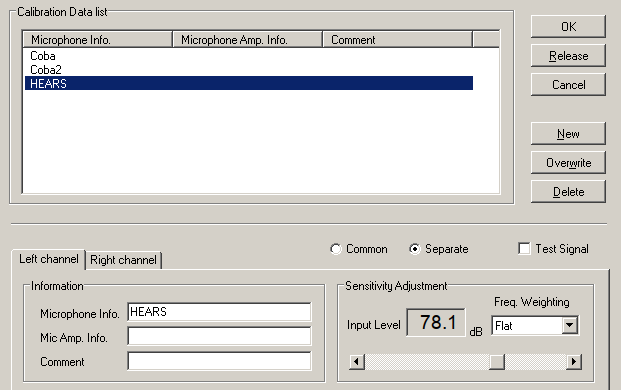
\includegraphics[width=200pt]{images/kalib}
			\caption{Jendela Kalibrasi}
		\end{figure}
		\item Masukkan microphone ke kalibrator.
		\begin{figure}[!ht]
			\centering
			\begin{subfigure}[b]{0.2\textwidth}
				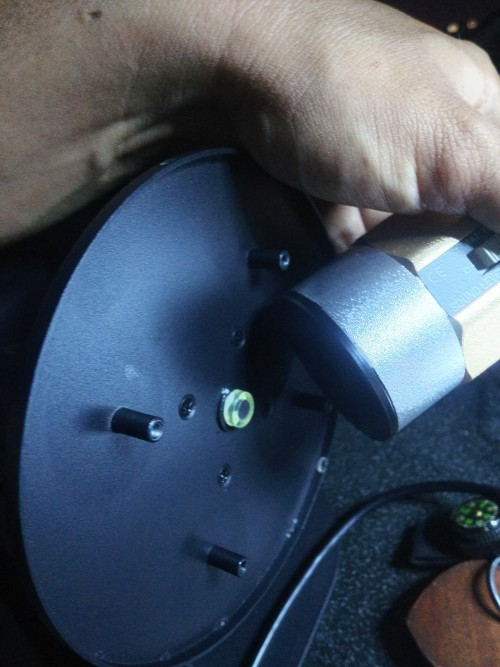
\includegraphics[width=\textwidth]{images/ears_calib0}
			\end{subfigure}
			\begin{subfigure}[b]{0.2\textwidth}
				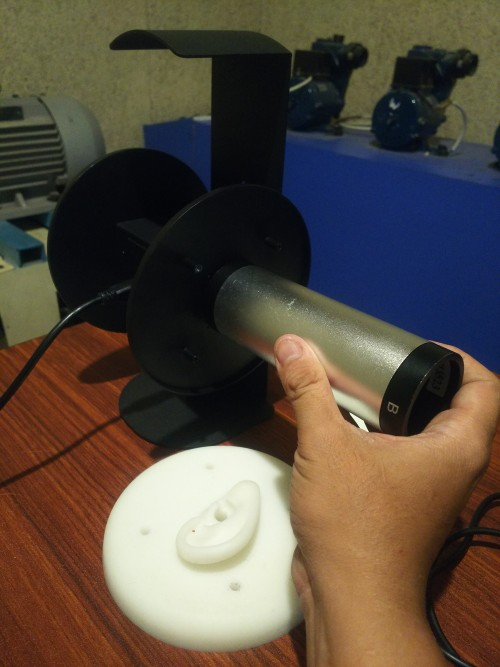
\includegraphics[width=\textwidth]{images/ears_calib1}
			\end{subfigure}
			\caption{Kalibrasi EARS}
		\end{figure}
		\item Geser slider kalibrasi hingga menunjukkan angka 114dB
		\item Ulangi untuk microphone di sisi lainnya.
		\item Beri nama pada \textbf{Microphone Info} dan klik \textbf{New} untuk menyimpan.
	\end{enumerate}

	\subsubsection{Mic}
	
	Menyusul
	
	\subsection{Pengukuran latar}
	
	Pengukuran latar dilakukan di kedua paket instrumen dan dibandingkan dengan hasil ukur SLM.
	
	\subsubsection{EARS}
	
	Hasil pengukuran SLM menunjukkan kondisi loudness latar berkisar pada 25 dB.
	File CSV pengukuran selama 10 detik dapat dilihat disini:
	\begin{itemize}
		\item \url{https://github.com/mekatronik-achmadi/elitech/blob/master/data/preparation/SNGL-MANU_-B706-210928132100.csv}
		\item \url{https://github.com/mekatronik-achmadi/elitech/blob/master/data/preparation/SNGL-MANU_-B707-210928135234.csv}
	\end{itemize}
	
	\newpage
	\begin{figure}[!ht]
		\centering
		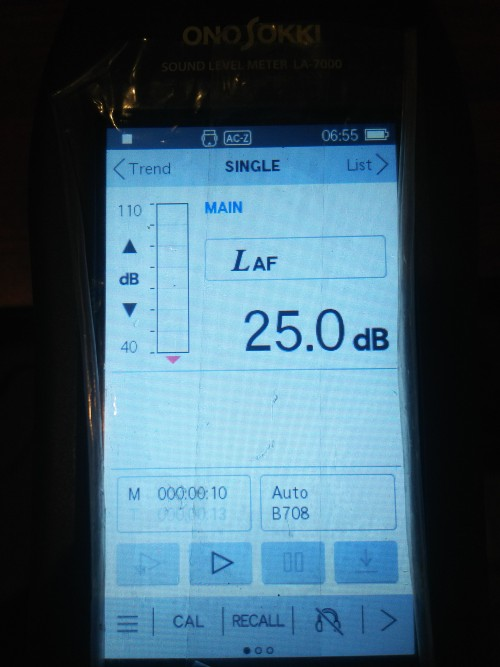
\includegraphics[width=125pt]{images/slm_latar}
		\caption{Pengukuran Latar dengan SLM}
	\end{figure}

	Sedangkan untuk EARS digunakan fitur \textbf{Record} pada FFT Analyzer di 1/3 Octave Band
	dalam durasi 30 detik dengan interval 1 detik setiap sampling.
	
	\begin{figure}[!ht]
		\centering
		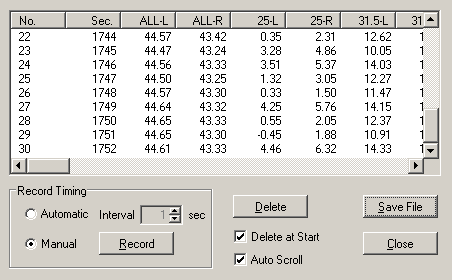
\includegraphics[width=200pt]{images/datarec}
		\caption{Contoh Rekaman Data}
	\end{figure}

	File CSV hasil pengukuran dapat dilihat di tautan:
	\url{https://github.com/mekatronik-achmadi/elitech/blob/master/data/preparation/EARS_Background.csv}
	
	\subsubsection{Perbandingan Hasil SLM-EARS}
	
	Dengan memperhatikan antara hasil \textit{record} EARS dan SLM,
	terlihat perbedaan nilai antara pembacaan SLM dan nilai akumulasi frekuensi (ALL).
	Hal ini disebabkan nilai frekuensi ALL adalah nilai log dari jumlah anti-log setiap spektrum frekuensi.
	Dalam ekspresi matematis:
	
	\[L_{sum} = \log (\sum 10^{L_i/10}) \]
	
	dengan \(L_i\) sebagai nilai dB SPL setiap spektrum frekuensi.
	
	Untuk mempermudah perhitungan, digunakan fungsi Python Numpy.
	
	\begin{minted}[frame=lines,framesep=2mm,fontsize=\tiny,bgcolor=LightGray]{python}
def SplAll(dataIn):
	freqSum = 0
	for i in range(len(dataIn)):
		valeach = np.power(10,dataIn[i]/10)
		freqSum = freqSum + valeach
		freqAll = 10* np.log10(freqSum)
	
	return freqAll
	\end{minted}

	kemudian import data menggunakan Python Pandas dan kalkulasi baris pertama hingga frekuensi 12500 Hz (array index 59)
	
	\begin{minted}[frame=lines,framesep=2mm,fontsize=\tiny,bgcolor=LightGray]{python}
data = pd.read_csv('./EARS_Background.csv')
Lsum = SplAll(data.iloc[0,4:59:2])
	\end{minted}

	dan nilai Lsum akan menunjukkan nilai mendekati frekuensi ALL pada record (43.99 dB).
	
	\newpage
	Sebagai pembanding, jika nilai spektrum di rata-rata menggunakan fungsi Numpy Python:
	
	\begin{minted}[frame=lines,framesep=2mm,fontsize=\tiny,bgcolor=LightGray]{python}
Lavg = np.average(data.iloc[0,4:59:2])
	\end{minted}

	dan nilai Lavg akan menunjukkan nilai mendekati hasil pembacaan SLM (24.96 dB)
	
	Memperhatikan nilai akumulasi frekuensi (43.99 dB) dan rata-rata frekuensi (24.96 dB),
	maka dipilih metode rata-rata untuk penentuan nilai SPL pada pengujian Speech dan Wishper.
	
	Kesimpulan yang digunakan sebagai nilai loudness latar adalah \textbf{25 dB SPL}.
	Skrip Python untuk pengolahan data dapat dilihat di tautan:\\
	\url{https://github.com/mekatronik-achmadi/elitech/blob/master/data/preparation/EARS_Background.ipynb}
	
	\subsubsection{Mic}
	
	Menyusul
	
	\subsubsection{Perbandingan Hasil SLM-Mic}
	
	Menyusul
	
	%%%%%%%%%%%%%%%%%%%%%%%%%%%%%%%%%%%%%%%%%%%%%%%%%%%%%%%%%%%%%%%%%
	
	\newpage
	\section{Hasil Pengukuran}
	
	
\end{document}